

\lstset{language=C,
	keywordstyle=\color{darkred},
	deletekeywords={int,while},
	morekeywords={critical,pragma,parallel,omp},
	commentstyle=\color{darkgray},
	stringstyle=\color{darkgreen},
	basicstyle=\small\sffamily\upshape,
	escapeinside={(*}{*)},  
	backgroundcolor=\color{lightgray}
	}

Between 1997 and 2005, the Laboratoire G\'enie de Production of the National Engineering School of Tarbes developed an Explicit Finite Elements Code for the numerical simulation of the behavior of mechanical structures subjected to impacts in large thermomechanical deformations: the DynELA FEM code. This academic FEM code has been used in support of different Ph.D. theses and several scientific publications \cite{Pantale:2002,Pantale:2004,Menanteau:2006,Nistor:2007,Nistor:2008} among which, one \cite{Pantale:2005} was focused on the parallelization of the DynELA FEM code using the OpenMP library. The purpose of this paper is to present the steps that were necessary to allow the reproduction of the results presented in the original article \cite{Pantale:2005} using the 2005 version of the DynELA code.

\section{Historical context}

During my thesis work (1992-95), discussions with my thesis supervisor led me to propose a new research theme focused on the numerical development of a FEM code for the study of large deformations: the DynELA FEM code. FEM codes are typically written in procedural programming languages such as Fortran or C. Adding new features to already very long programs requires programmers to work with a complexity that increases exponentially with the initial size of the code. Object-Oriented Design and Programming (OOP) methods are better suited to large-scale developments. The abstraction allowed by OOP allows the developer to better organize the architecture of the program and to anticipate future developments. The preferred programming language in the Finite Element community was C++ at the date of the original publication (maybe because of novelty in 1990-2000), and it was our choice for the numerical implementation of the FEM code DynELA. The main characteristics of this code are an explicit integration scheme and a formulation in large deformations, an Object-Oriented approach for the numerical implementation in C++, and an open code architecture based on own developments and use of open-source libraries.

This work was mainly motivated by the fact that the development of a FEM code allows a very important personal intellectual enrichment. The numerical developments allow us to deepen the knowledge in the field of mechanics of large deformations since one is forced to master the theory to be able to implement it numerically. It is a phase of consolidation of knowledge directly through experience, certainly more delicate, but much more thorough.

\subsection{Architecture of the FEM code}

In a finite element code development, the first step is defining a set of basic libraries for data management (in the form of lists, stacks, ...) as well as the mathematical libraries adapted to the modeling cases encountered. Our choice was to develop entirely the set of basic libraries and to encapsulate a part of the Lapack \cite{Lapack:1999} mathematical library to develop new matrix and tensor classes because no mathematical library was available for this purpose. For example, classical mathematical libraries do not include the notion of 4th-order tensor. The FEM code DynELA is composed of a set of separate libraries and executable files that complete particular tasks. A simplified list of these libraries is given below:
\begin{itemize}
\item basicTools: basic library which contains the basic classes of DynELA.
\item linearAlgebra: algebraic operations library. It defines in particular the notions of vectors, matrices, tensors, and mathematical functions. It encapsulates part of the Lapack and Blas libraries.
\item interpretor: library that defines the interpreted command language of DynELA. It was one of the strong points of the original software.
\item femLibrary : finite element computation library (it is the heart of the finite element solver).
\end{itemize}
From these various libraries, we created a set of executable programs that correspond to the various modules of the FEM code: the finite element solver, the graphics post-processor, the curve analysis program, the language generator, etc...

\subsection{Specifics of the DynELA FEM code}
In terms of size of development, one can estimate the number of C++ lines of code for the different modules as follows:
\begin{itemize}
\item Command interpreter: 10,000 lines of C++ code, Flex and Bison \cite{Levine:2009}
\item Graphics post-processor: 20,000 lines of C++ code
\item Finite element solver: 80,000 lines of C++ code.
\end{itemize}

\subsubsection{Command interpreter}
One of the key decisions in the development of a FEM code lies in the way the user specifies the data of a model. Several alternatives are possible. Some codes privilege the use of a graphical interface allowing the user to build step by step the numerical model, others use a command file that the user edits externally. We adopted an advanced command language as the means of defining a numerical model. 

The trend at the time of this work was towards the development of command languages for driving simulation codes to replace the command files inherited from the punched card era that were still found in many numerical codes. Concerning the DynELA FEM code, the choice was a specific lexical and grammatical parser developed using standard Flex and Bison tools. Generally speaking, this command file has a syntax close to the C++ language and allows the manipulation of object-oriented data, the writing of tests and loops. 
 
\subsubsection{Graphics post-processor}

The numerical results are analyzed by means of a graphical post-processor specially developed for the DynELA FEM code. The 3D graphical part uses OpenGL formalism, and the interface is constructed using the QT graphical library. The porting of the post-processor to the new architecture did not pose any problems concerning the OpenGL library, on the other hand, concerning the QT library, the initial version was based on QT-3, but the porting to QT-4 was carried out between 2005 and 2010 for the continuity of the work related to the various Ph.D. theses in progress over this period. The version of the graphic post-processor used in this work to analyze the results and produce outputs is therefore the one developed in 2010.

\subsubsection{Finite element solver}

The finite element solver used in this work is version v.1.0 developed in the laboratory between 1996 and 2005, the date of publication of the referenced paper. The finite element solver subsequently evolved after 2005 and up to 2010, but \textbf{since this is after the publication of the referenced paper, it has not been used for this work}. Moreover, in 2005, there were 2 versions of the FEM code: a \textbf{standard 1.0 version} (the one that has continued to evolve) and a \textbf{parallel beta version} (not modified afterwards and completely frozen in 2005), and it is the latter that was used in this work.

\subsection{Computational context of the original publication}
The publication selected for this work \cite{Pantale:2005} used a Compaq Proliant 8000 SMP machine running under Linux Redhat 8.0 environment. This machine, shown in Figure \ref{proliant} was equipped with 8 32-bits Intel Xeon PIII 550/2Mb processors around a 5GB shared main memory. 
\begin{figure}[h] 
  \centering
  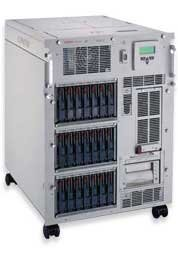
\includegraphics[width=0.3\textwidth]{./8000_photo.jpg}
  \caption{The Compaq Proliant 8000 SMP machine}
  \label{proliant}
\end{figure}
The source code was compiled with the Intel Cpp 7.1 compiler without optimization in order to be able to compare the different parallelization techniques without any influence of the compiler. The OpenMP standard was chosen for code parallelization.

\section{Retrieval of the software}

Between 2010 and 2018, the research activities put aside the development of this Finite Element code, but, since september 2018, a new version in C++ and Python was started to restore this numerical tool and allow new developments. This new version is based on the latest stable version (the 2010 version) but this is another story, and only the Timer class of this modern version was used for this paper to replace the old problematic class dedicated to processor time measures as presented further.

\subsection{Finding the source code}

First of all, finding the complete source code of the version used for publication was not an easy task. Indeed, the different versions were developed and archived on various digital supports (floppy disks, CDROM, floppy ZIP, ...)\footnote{Things that have more or less disappeared by now...}, the incremental numbering was not always respected, and by bad luck, the Proliant server which contained the very last version used for the production of the scientific publication was scrapped without saving all the sources of the code (or else, the backup has been lost since). Only the modified files concerning the standard 1.0 version were found in a backup hard-disk. It was therefore possible to rebuild a version as close as possible to the final version based on the standard 1.0 version by merging the source files of the parallel version. The first point that emerges from the difficulties related to the recovery of old source code concerns the need to improve the procedures for archiving the source code of the software developped in our laboratory\footnote{As a result of this experience, we are going to set up a committee within the laboratory to reflect on the sustainability of the research data produced by the laboratory.}. I detail hereafter, the procedure used to rebuild a working set of source files:
\begin{itemize}
\item get the version 1.0 set of sources files from a backup dated 2004, those were on a backup of my desktop computer where I never tested the parallel version of the code,
\item by hand, and one by one, merge the different updated files from the parallel version backup into the set of source files of version 1.0,
\item install the already compiled post-processor from the 2010 version of the code for visualization of the results and production of output results,
\item replace the processor time measurement class by the one from the newest version of DynELA, as presented in the next paragraph.
\end{itemize}

Therefore, the major change made to the core of the Finite Element code concerns the subroutine for execution time measurement used to know the times spent in the various parts of the program. In fact, during the first tests, the times reported by the original class were outliers. We therefore decided to simply replace the version 1.0 time measurement class by the one developed for the new version of the DynELA code. Hopefully they were directly compatible to each other, because they were both developed with the same philosophy. The measurement points in the code were thus modified to take into account this new class for measuring processor times.

\subsection{Hardware used for the reproduction}

As the machine used at the time of the publication of the proposed paper (in 2005) has been scrapped since then, the implementation of this work was done on a Dell R730 server equipped with 2 64-bits Intel Xeon E5-2650 v4, 2.20GHz processors (each with 12 cores) and 96GB of RAM. This server runs under Ubuntu Bionic 18.04.4 LTS with a 4.15.0-76 kernel. 

The hardware configuration is therefore clearly different from the one used in the original article, so we can expect that, if the Finite Element code runs correctly and gives numerical results in agreement with those obtained in the original paper, as it will be presented further, the performance and the behavior concerning code parallelization will differ due to the change in processor architecture, memory and especially the evolution of the Operating System.

\section{Compilation, update of the code and benchmarks}

As presented above, the DynELA code is composed of several thousand C++ lines of code located in an organized tree structure, which more or less facilitated the compilation procedure. The compilation of the various modules must be chained directory by directory, a library being compiled in each main sub-directory. The number of dependencies and the complexity of the code tree made it necessary to use a tool not used at the time of the initial development, the CMake \cite{CMake} utility for the generation of different Makefiles in the source directories. At the time of development, the Makefiles were handwritten, and the compilation of the sources was done directly in the source directories themselves (which is not a good thing to do), we had a mixture of C++ sources, headers and compiled objects in the same directories.

So the first step was to reorganize the sources on one side, a Build tree in a separate directory and to create a set of compilation directives for the CMake utility. Of course, we also had to take into account the required dependencies concerning external libraries: Flex and Bison \cite{Levine:2009} mainly, but this phase does not pose any problem as these libraries are standard on Linux, and one just has to install them using an appropriate ubuntu package. The old Makefiles contained all the needed information concerning the required libraries.

\subsection{Compilation of the code}

The compilation of the DynELA code is done using the standard compiler on Ubuntu 18.04.4 LTS: the C++ 7.4.0. Flex and Bison versions are 2.6.4 and 3.0.4 respectively. The parallelization is done using the -fopenmp compiler option and the OpenMP parallelization libraries is provided by the gcc-7 library.

During the compilation of the code, several warning messages are generated (mainly concerning functions not explicitly defined at compile time and due to evolution in the C++ standard within the last 15 years), however these have been ignored and do not seem to be detrimental to the proper compilation of the source code or its execution. The compilation part of the Lapack and Blas mathematical libraries is done without any problem (note that these libraries have been translated from Fortran by the f2c utility and are part of the CLAPACK and CBLAS packages).

\subsection{Comparison of results vs. the original paper}

\subsubsection{Comparison of numerical results}\label{Ptensile}

After the compilation phase, the first operation was to rerun the simulations presented in the initial publication and to compare the results. Figure \ref{strain} shows the results for the numerical simulation, using 4 processors, of a dynamic tensile test with on the left side the initial mesh, and on the right side the deformed plastic strain contourplot at the end of the simulation, corresponding to Figure 9, page 370, of the original paper \cite{Pantale:2005}.

\begin{figure}[h!] 
  \centering
  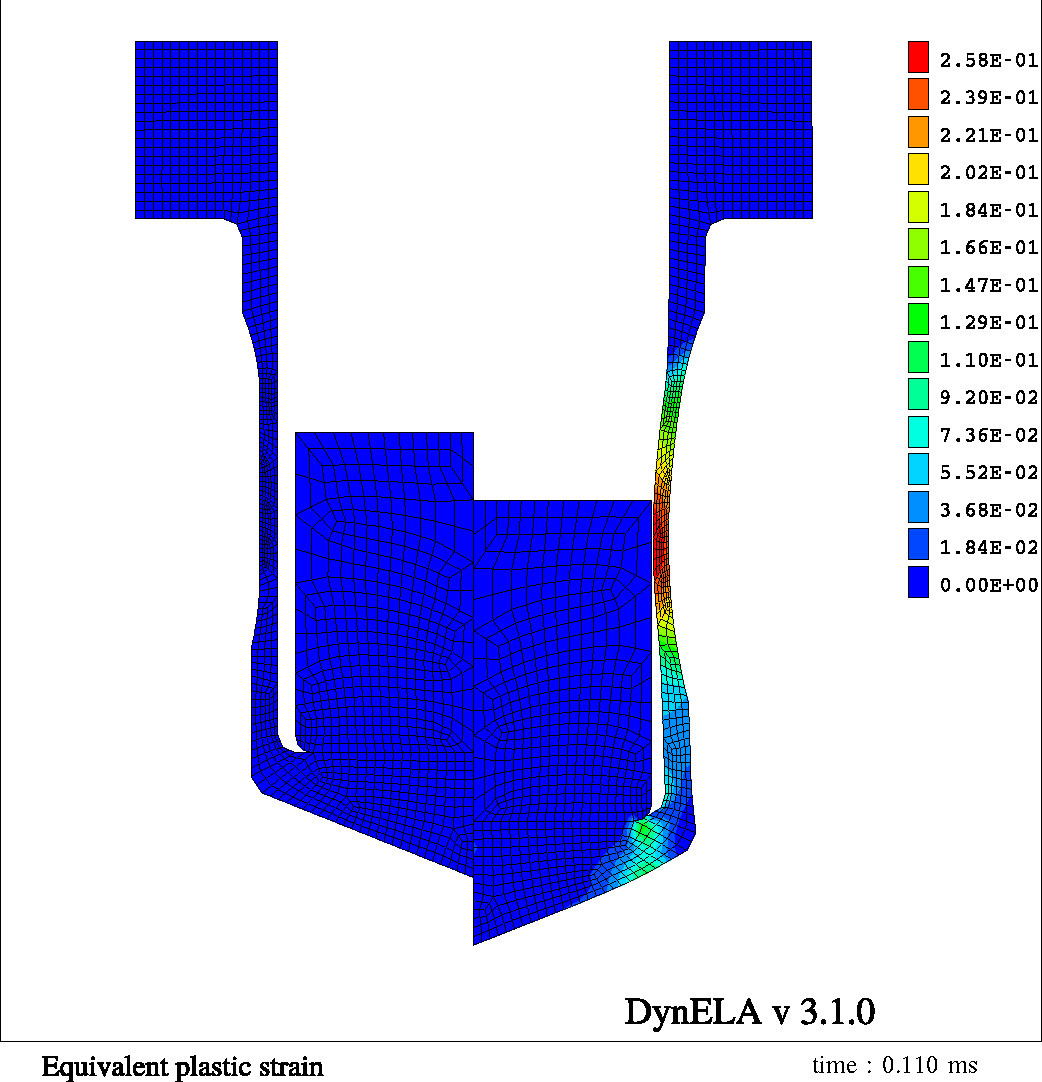
\includegraphics[width=0.6\textwidth]{./strain.pdf}
  \caption{Dynamic traction: initial mesh and equivalent plastic strain contourplot}
  \label{strain}
\end{figure}

We find good agreement between the two simulations thus confirming behaviour of the FEM code. The values are not the same, but the difference is very small. Maybe they are linked to some accumulation of floating-point errors (explicit integration scheme in FEM are very sensitive to this) since we have a 32-bits processor on one hand and a 64-bits processor on the other hand. Other comparisons confirm that the code does indeed give the same numerical results as in its 2005 version, but are not reported in this article. The good agreement between the two versions confirm the correct behavior of the code between its two deployments 15 years apart. No crashes of the computation code, segmentation fault type problems, or other problems that could suggest an instability of the code structure were observed. Only abrupt stoppages due to data errors were encountered, but they are similar to those obtained in the standard 1.0 version (so the errors also are reproducible).

\subsubsection{Internal forces computation parallelization}

The main subject of the original publication in 2005 was the parallelization of the DynELA code and \textbf{the influence of the strategies on the Speedup}. We therefore rerun the numerical experiments with the different code parallelization strategies and tried to replicate the results obtained in 2005. We will focus on the parallelization of the computation of the internal forces (presented in paragraph 4.3, page 367 of \cite{Pantale:2005}) for the Taylor test with a mesh consisting of 6500 finite elements (as presented in paragraph 4.2 page 367 of \cite{Pantale:2005}). 

This computation is the most processor intensive part of the FEM code. In Listing \ref{listing}, the method \textbf{computeInternalForce} is applied on each element of the mesh and returns the internal force vector resulting from the integration over the element. The \textbf{gatherFrom} operation assembles the resulting element internal force vector into the global internal force vector of the structure.

\begin{lstlisting}[label=listing,caption={Internal forces computation (standard version)},captionpos=b]
Vector Fint;
for (int elm = 0; elm < elements.size (); elm++) {
   Vector FintElm;
   elements(elm).computeInternalForces (FintElm);
   Fint.gatherFrom (FintElm, elements(elm));
}
\end{lstlisting}

In the original paper, 4 parallelization methods were compared, out of the 8 methods available in the DynELA code. All simulations were redone with these 8 parallelization methods, and the results in terms of speedup for the 4 ones corresponding to \cite{Pantale:2005}, and described hereafter, are reported in Figure \ref{speedup}.
\begin{figure}[h!] 
  \centering
  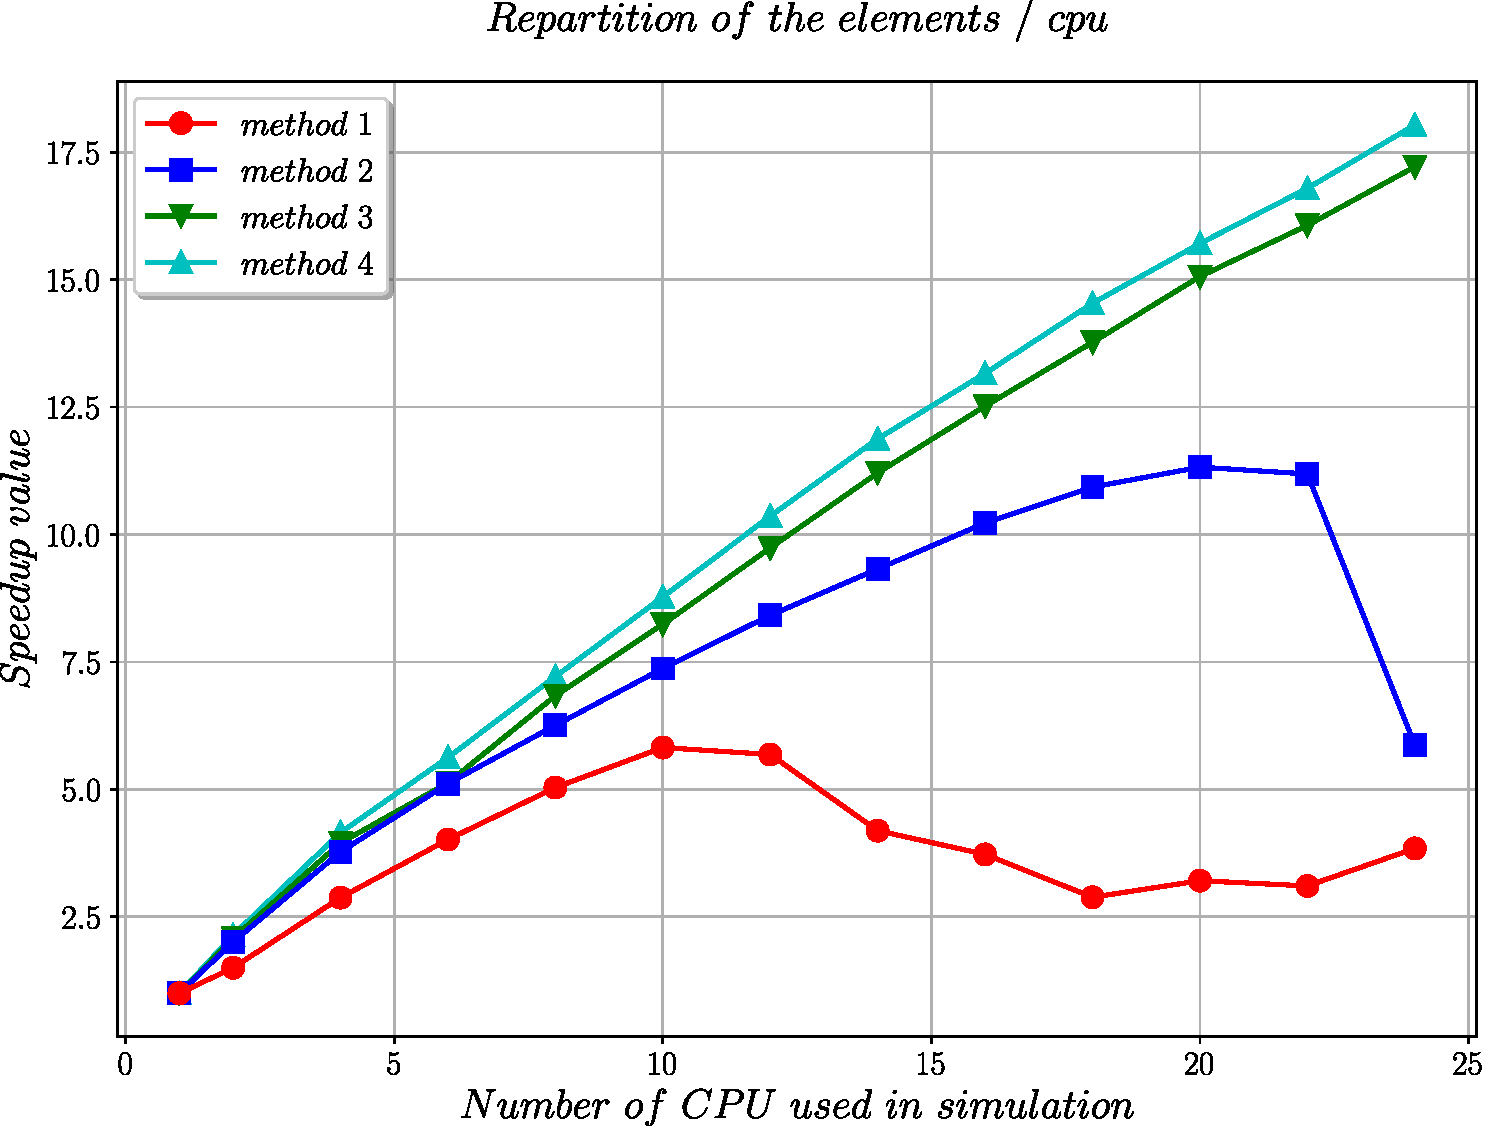
\includegraphics[width=0.75\textwidth]{./speedup.pdf}
  \caption{Speedup of the $\protect\overrightarrow{F^{int}}$ computation for various implementations}
  \label{speedup}
\end{figure}

\begin{enumerate}
\item Method 1, presented in Listing \ref{method1}, uses a parallel for directive for the main loop and share the $\overrightarrow{F^{int}}$ vector among the threads. A critical directive is placed just before the gatherFrom operation because $\overrightarrow{F^{int}}$ is a shared variable. The results plotted in red in Figure \ref{speedup} shows a rapid collapse of the performance of the parallelization algorithm beyond 10 processors.
\lstinputlisting[label=method1, caption=Internal forces computation with method 1]{method1.C}
\item Method 2, presented in Listing \ref{method2}, uses a parallel region directive. In this parallel region, all threads access a shared list of elements to treat until empty. The $\overrightarrow{F^{int}}$ vector is declared as private. Both main operations are treated without the need for any critical directive. At the end of the process, all processors are used together to assemble the local copies of the $\overrightarrow{F^{int}}$ vector into a global one. The results plotted in blue in Figure \ref{speedup} shows a rapid collapse of the performance of the parallelization algorithm when the number of processor used for the simulation approaches the maximum number of processors of the server.
\lstinputlisting[label=method2, caption=Internal forces computation with method 2]{method2.C}
\item Method 3, presented in Listing \ref{method3}, is similar to the previous one except that each thread has a predetermined equal number of elements to treat. Therefore, we avoid the use of a shared list (as in method 2), and each processor operates on a block of elements. A dedicated class Jobs is used to manage the dispatching of the elements over the processors. In contrast to the previous method, in this case, there is an increase in performance regardless of the number of processors used as reported by the green curve in Figure \ref{speedup}.
\lstinputlisting[label=method3, caption=Internal forces computation with method 3]{method3.C}
\item Method 4, is the same as method 3 except that we use the dynamic load balance operator presented in \cite{Pantale:2005} after the gather block as presented in Listing \ref{method4}. As in the previous case, in this case, there is also an increasing gain in performance regardless of the number of processors used, but this gain is greater than that of method 3 (see the cyan curve in Figure \ref{speedup}).
\lstinputlisting[label=method4, caption=Internal forces computation with method 4]{method4.C}
\end{enumerate}

The results of Figure \ref{speedup} should be compared with Figure 7 page 369 of \cite{Pantale:2005} since the current server has 24 processors, we were able to extend the analysis beyond the 8 processors originally used. The speedups obtained in the current version are globally lower over beyond 8 processors, but this can be explained by:
\begin{itemize}
\item the fact that the OS used is better at multitasking than the one used in 2005, which means that the machine has a different workload,
\item the hardware architecture also differs (the Compaq Proliant machine had 8 independent 32-bits processors, while the current one 2 multi-core 64-bits processors), the working disks are now on another server, and we use an NFS protocol that can have an impact on code parallelization performance,
\item the numerical model is identical to the one used in 2005, but in order to have a significant gain on a large number of processors (range beyond 8), the size of the model would have to be larger in order to ensure that each processor can handle a sufficient number of elements to justify the use of parallelization (roughly speaking, fork and join times become non-negligible when the load/processor decreases). But this would have changed with regard to the original test published which is outside the scope of the reproducibility challenge associated with this work.
\end{itemize}
Nevertheless, and despite these differences, we can notice that the current version replicates the trends seen in 2005 and that method 4 provides more speedup as a function of the number of processors while method 1 shows its limits very quickly. The same conclusions can, therefore, be drawn concerning the parallelization of the code as those obtained in the article \cite{Pantale:2005}, which shows the replicability of the results.

\subsubsection{The load balancing algorithm}

In this last part, we compare the results obtained by the load balancing algorithm in the computation of the internal force vector. This algorithm seeks to minimize the waiting time of the different processors in the parallel internal force vector evaluation phase by dynamically changing the number of elements allocated to each processor during the computation. The original results are presented in paragraph 5 on page 371 of the article \cite{Pantale:2005}.

This simulation uses the test case of the tensile test presented in paragraph \ref{Ptensile}. Figure \ref{spacethreads} shows the spatial distribution of the elements for the numerical simulation of the tensile test on 4 processors over time, respectively, at the beginning of the simulation (left part of the figure), at 50\% of the calculation (middle part of the figure) and at the end of the calculation (right part of the figure). Obviously, the comparison with Figure 11, page 372 of the article \cite{Pantale:2005} shows differences concerning the localization of the elements with respect to the different processors, as well as Figure \ref{timethreads}, to be compared with Figure 12 page 373 of the article \cite{Pantale:2005}. Nevertheless, the same global remarks can be made about the load balancing algorithm used in the DynELA code. It is therefore clear that the number of elements held in each processor evolves over time in order to balance loads of each processor during the calculation.

In conclusion, we can say that even if the results in terms of parallelization gain, localization of the elements with respect to the different processors, are different, the global behavior of the DynELA code is consistent. The results of the numerical simulations are in agreement with the results obtained in the simulations carried out in 2005.

\begin{figure}[h!] 
  \centering
  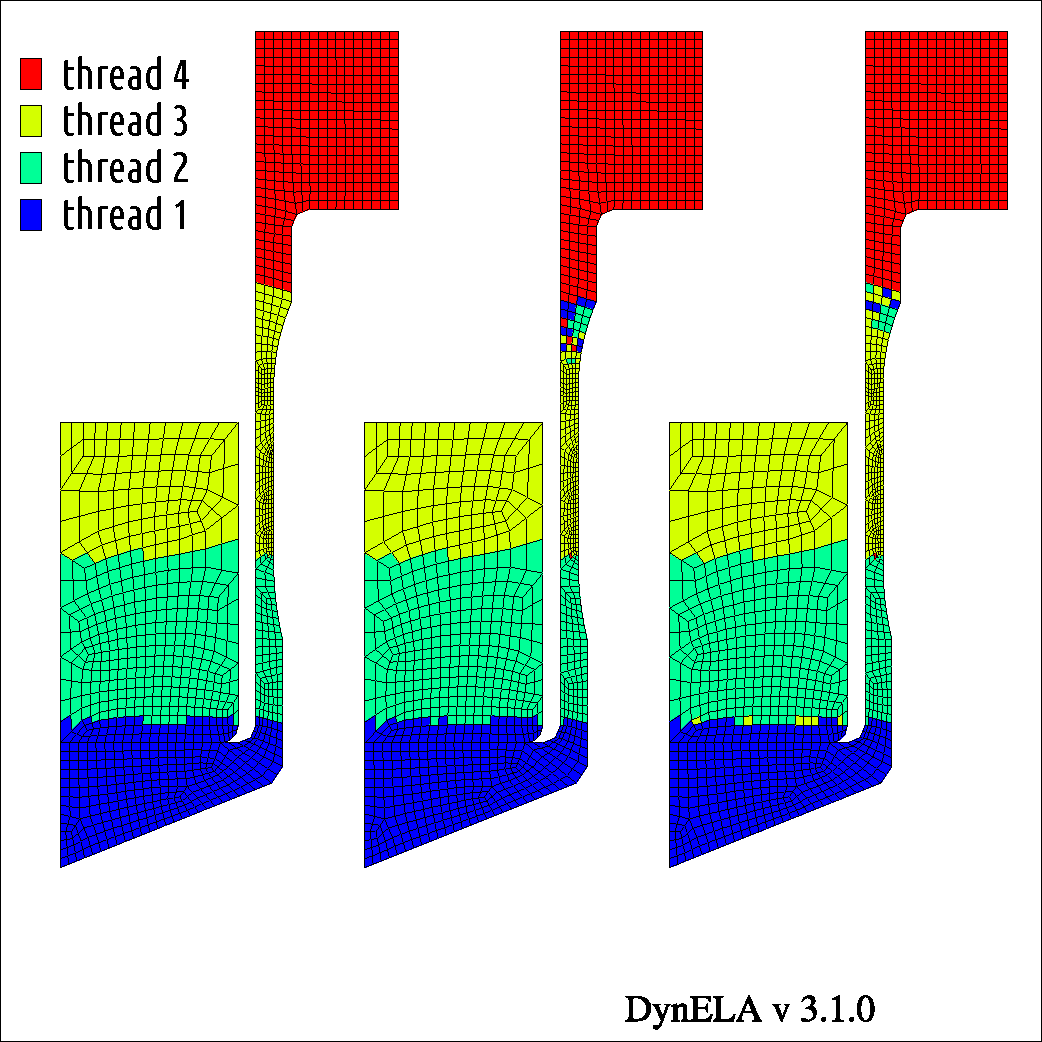
\includegraphics[width=0.6\textwidth]{./spacethreads.pdf}
  \caption{Spatial distribution of the elements during computation}
  \label{spacethreads}
\end{figure}

\begin{figure}[h!] 
  \centering
  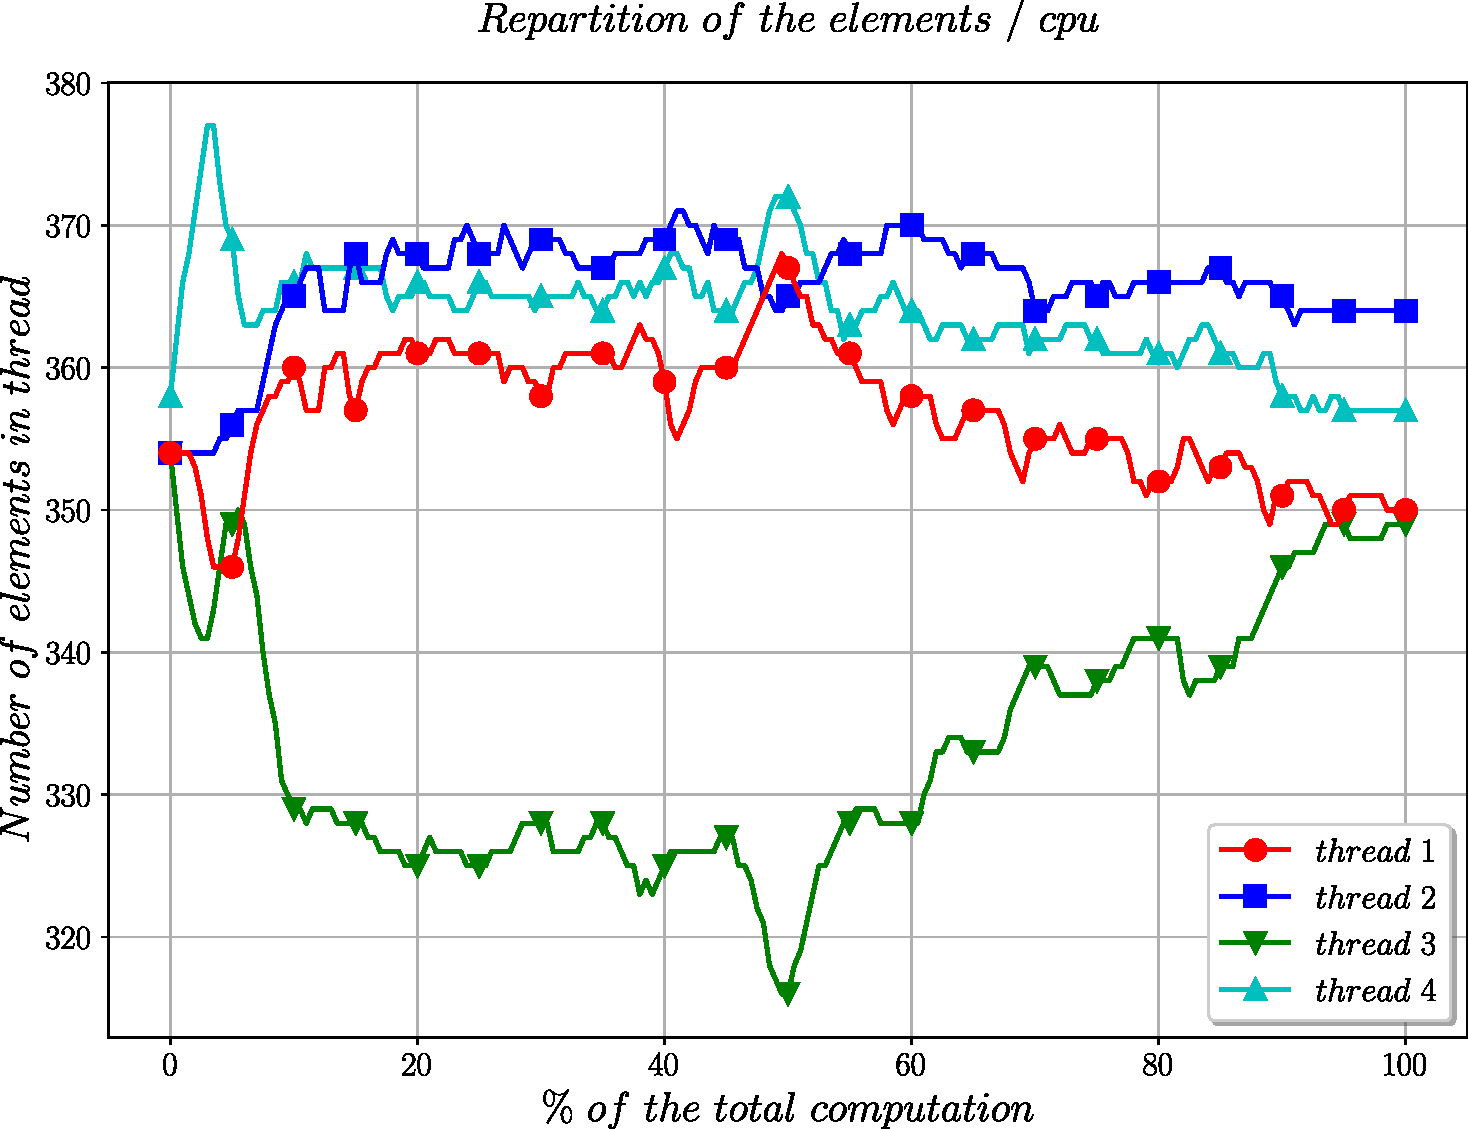
\includegraphics[width=0.75\textwidth]{./timethreads.pdf}
  \caption{Distribution of the elements during computation}
  \label{timethreads}
\end{figure}

\section {Conclusions}

Fifteen years after the publication of the original article \cite{Pantale:2005} concerning the parallelization of the DynELA Finite Element code, the results were found to be reproducible and replicable. It is still possible, with some adjustments, to recompile the code as proposed in 2005 (about 2 days of work were necessary to be able to complete the compilation of the DynELA code). The execution of the code on modern computing architectures did not pose any problems, as no crashes were experienced during the numerical simulations and the use of the code. The results in terms of performance are consistent with the results obtained 15 years ago, taking into account the radical change in hardware architecture for the execution of this Finite Element code.

This paper deals with both replication (applies to the analysis of multi-threading strategies), and reproduction (applies to the benchmark on dynamic-traction simulation) of the original article \cite{Pantale:2005}. We found that, even if the architecture of the processors differ (32-bits single core on one hand and 64-bits multi-core on the other hand), the results are reproducible concerning the numerical results and replicable concerning the multi-threading strategies with OpenMP where method 1 saturates and does not scale, and method 4 scales the best with an increasing number of processors.

One of the consequences of participating in this challenge is to have been able to 'find' the source code of the original publication. So, the work is reproducible now, with the code made available with this work. The future will tell us if, in a few years, these results will still be replicable/reproducible on future hardware architectures.

